%%%%%%%%%%%%%%%%%%%%%%%%%%%%%%%%%%%%%%%%%
% fphw Assignment
% LaTeX Template
% Version 1.0 (27/04/2019)
%
% This template originates from:
% https://www.LaTeXTemplates.com
%
% Authors:
% Class by Felipe Portales-Oliva (f.portales.oliva@gmail.com) with template 
% content and modifications by Vel (vel@LaTeXTemplates.com)
%
% Template (this file) License:
% CC BY-NC-SA 3.0 (http://creativecommons.org/licenses/by-nc-sa/3.0/)
%
%%%%%%%%%%%%%%%%%%%%%%%%%%%%%%%%%%%%%%%%%

%----------------------------------------------------------------------------------------
%	PACKAGES AND OTHER DOCUMENT CONFIGURATIONS
%----------------------------------------------------------------------------------------

\documentclass[
	12pt, % Default font size, values between 10pt-12pt are allowed
	%letterpaper, % Uncomment for US letter paper size
	%spanish, % Uncomment for Spanish
]{fphw}

% Template-specific packages
\usepackage[utf8]{inputenc} % Required for inputting international characters
\usepackage[T1]{fontenc} % Output font encoding for international characters
%\usepackage{mathpazo} % Use the Palatino font
\usepackage{times}

\usepackage{graphicx} % Required for including images

\usepackage{booktabs} % Required for better horizontal rules in tables

\usepackage{listings} % Required for insertion of code

\usepackage{enumerate} % To modify the enumerate environment

\usepackage{amsfonts,amssymb}

%----------------------------------------------------------------------------------------
%	ASSIGNMENT INFORMATION
%----------------------------------------------------------------------------------------

\title{Homework \#1} % Assignment title

\author{2001111696 Zhaohui Huang} % Student name

\date{\today} % Due date

\institute{Peking University} % Institute or school name

\class{Optimization Methods in Machine Learning} % Course or class name

\professor{Prof. Zhouchen Lin} % Professor or teacher in charge of the assignment

%----------------------------------------------------------------------------------------

\begin{document}

\maketitle % Output the assignment title, created automatically using the information in the custom commands above

%----------------------------------------------------------------------------------------
%	ASSIGNMENT CONTENT
%----------------------------------------------------------------------------------------

\section*{Question 1}

\begin{problem}
	The no-free-lunch (NFL) theorem is actually quite general. Give another instance that you think the NFL theorem holds.
\end{problem}

%------------------------------------------------

\subsection*{Answer}

\begin{itemize}
	\item While the airplane is less time-consuming than any other transportations, e.g., cars, high-speed railway, for a long journey, they can outperform airplane for different specific situations.
	\item All possible travel cases taken into consideration, all transportations are necessary and perform on average equally well.
	\item There is no universally better transportation exist.
\end{itemize}

%----------------------------------------------------------------------------------------

\section*{Question 2}

\begin{problem}
Write down an optimization problem, in the mathematical form, that you encounter in your daily life (do not copy from textbooks). Describe why you formulate in that way.
\end{problem}

%------------------------------------------------

\subsection*{Answer}
\ 
\newline
\noindent Suppose that I want to take several part-time jobs during my one-week holiday, the working time is expected to be less than 14 hours. There are two coffee houses and these two jobs as a waiter will cost me a deposit of 25/hour and 10/hour, respectively. The deposit will be paid before going to the job. I can afford no more than 300. The salary per hour in two coffee houses are 60/hour and 40/hour, respectively. How can I distribute my time to earn more money?\\

Sol: Let x and y be the working time at two coffee houses, then 
$$min_{x,y} f(x,y)=35x+30y$$
$$s.t. x+y \leq 14,25x+10y \leq 300$$

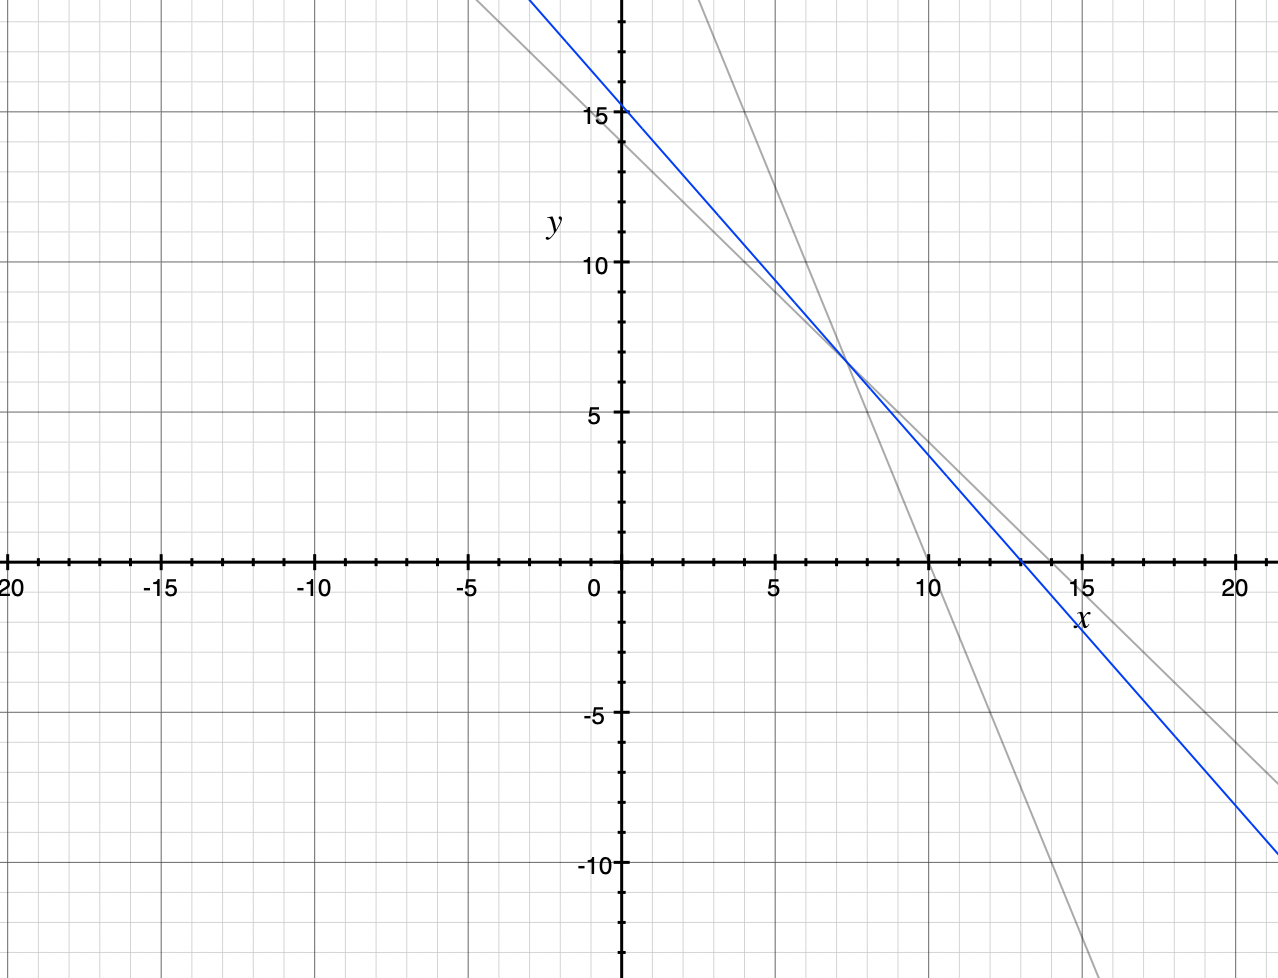
\includegraphics[scale=0.6]{op.png}

By simple linear programming, we can calculate $$x_m=\frac{22}{3}, y_m=\frac{20}{3}, f_m=\frac{1370}{3}$$
$\hfill \square$
%----------------------------------------------------------------------------------------

\section*{Question 3}

\begin{problem}
	Judge the properties of the following sets (openess, closeness, boundedness, compactness) and give their interiors, closures, and boundaries:
	
	\medskip
	
	\begin{enumerate}[a. ]
		\item $\mathcal{C}_1=\emptyset$.
		\item $\mathcal{C}_2=\mathbb{R}^n$.
		\item $\mathcal{C}_3=\{x|0\leq x<1\}\cup\{x|2\leq x \leq3\}\cup\{x|4<x \leq5\}$.
		\item $\mathcal{C}_4=\{(x,y)^T|x\geq 0,y> 0\}$.
		\item $\mathcal{C}_5=\{k|k\in \mathbb{Z}\}$.
		\item $\mathcal{C}_6=\{k^{-1}|k\in \mathbb{Z},k\neq 0\}$.
		\item $\mathcal{C}_7=\{(1/k,\sin{k})^T|k\in \mathbb{Z},k\neq 0\}$.
	
	\end{enumerate}
	
	\smallskip
\end{problem}

%------------------------------------------------

\subsection*{Answer} 

\begin{enumerate}[a. ]
		\item properties: openness, closeness, boundedness, compactness.\\
			interiors: $\emptyset$.\\
			closures: $\emptyset$.\\
			boundaries: $\emptyset$.
		\item properties: openness, closeness.\\
			interiors: $\mathbb{R}^n$.\\
			closures: $\mathbb{R}^n$.\\
			boundaries: $\emptyset$.
		\item properties: boundedness.\\
			interiors: $\{x|0< x< 1\}\cup\{x|2< x <3\}\cup\{x|4< x <5\}$.\\
			closures: $\{x|0\leq x\leq 1\}\cup\{x|2\leq x \leq3\}\cup\{x|4\leq x \leq5\}$.\\
			boundaries: $\{0,1,2,3,4,5\}$.
		\item properties: none.\\
			interiors: $\{(x,y)^T|x> 0,y> 0\}$.\\
			closures: $\{(x,y)^T|x\geq 0,y\geq 0\}$.\\
			boundaries: $\{(x,y)^T|xy\geq 0,x\geq 0,y\geq 0\}$.
		\item properties: closeness.\\
			interiors: $\emptyset$.\\
			closures: $\{k|k\in \mathbb{Z}\}$.\\
			boundaries: $\{k|k\in \mathbb{Z}\}$.
		\item properties: boundedness.\\
			interiors: $\emptyset$.\\
			closures: $\{k^{-1}|k\in \mathbb{Z},k\neq 0\}\cup \{0\}$.\\
			boundaries: $\{k^{-1}|k\in \mathbb{Z},k\neq 0\}\cup \{0\}$.
		\item properties: boundedness.\\
			interiors: $\emptyset$.\\
			closures: $\{(1/k,\sin{k})^T|k\in \mathbb{Z},k\neq 0\}\cup \{(0,\sin{k})^T|k\in \mathbb{Z},k\neq 0\}$.\\
			boundaries: $\{(1/k,\sin{k})^T|k\in \mathbb{Z},k\neq 0\}\cup \{(0,\sin{k})^T|k\in \mathbb{Z},k\neq 0\}$.
	
	\end{enumerate}


%----------------------------------------------------------------------------------------

\section*{Question 4}

\begin{problem}
Prove that a point $\mathbf{x}$ is a boundary point of $\mathcal{C}\subseteq \mathbb{R}^n$ iff for $\forall \epsilon >0$, there exists $\mathbf{y}\in \mathcal{C}$ and $\mathbf{z}\notin \mathcal{C}$ such that
$$\|\mathbf{y}-\mathbf{x}\|_2 \leq \epsilon, \quad \|\mathbf{z}-\mathbf{x}\|_2 \leq \epsilon.$$
\end{problem}

%------------------------------------------------

\subsection*{Answer}
\ 
\newline
\noindent Proof of Sufficiency:

for $\forall \epsilon > 0$, $B_{\epsilon}(\mathbf{x})=\{\mathbf{t}\in \mathbb{R}^n|\|\mathbf{t}-\mathbf{x}\|_2\leq \epsilon\}$, there exists $\mathbf{y}\in \mathcal{C}$ and $\mathbf{z}\notin \mathcal{C}$ such that $\mathbf{y},\mathbf{z}\in U(\mathbf{x},\epsilon)$, so $\mathbf{x}$ is a boundary point of $\mathcal{C}\subseteq \mathbb{R}^n$.\\

\noindent Proof of Necessity:

$\mathbf{x}$ is a boundary point of $\mathcal{C}\subseteq \mathbb{R}^n$, so $\mathbf{x} \notin \mathcal{C}^{\circ}$, i.e., $\forall \epsilon >0, B_{\epsilon}(\mathbf{x}) \not \subset \mathcal{C}$.
$\therefore \exists \mathbf{z} \notin \mathcal{C}$ but $\mathbf{z} \in B_{\epsilon}(\mathbf{x})$. Also, $\mathbf{x} \notin (\mathcal{C}^c)^{\circ}$, i.e., $\forall \epsilon >0, B_{\epsilon}(\mathbf{x}) \not \subset \mathcal{C}^c$.
$\therefore \exists \mathbf{y} \in \mathcal{C}$ but $\mathbf{y} \in B_{\epsilon}(\mathbf{x})$.So there exists $\mathbf{y}\in \mathcal{C}$ and $\mathbf{z}\notin \mathcal{C}$ such that
$$\|\mathbf{y}-\mathbf{x}\|_2 \leq \epsilon, \quad \|\mathbf{z}-\mathbf{x}\|_2 \leq \epsilon.$$
$\hfill \square$ 
%----------------------------------------------------------------------------------------

\section*{Question 5}

\begin{problem}
Prove that $\mathcal{C}\subseteq \mathbb{R}^n$ is closed iff it contains its boundary, and is open iff it contains no boundary points.
\end{problem}

%------------------------------------------------

\subsection*{Answer}

\begin{itemize}
	\item $\mathcal{C}\subseteq \mathbb{R}^n$ is closed iff it contains its boundary.
		\begin{itemize}
		\item Proof of Sufficiency:\\
		The boundary of $\mathcal{C} \subseteq \mathbf{R}^n$ is defined as $\partial \mathcal{C} =\overline{\mathcal{C}}\backslash \mathcal{C}^{\circ}$. $\because \mathcal{C}$ is closed, $\therefore \overline{\mathcal{C}}=\mathcal{C}$, $\partial \mathcal{C} =\mathcal{C}\backslash \mathcal{C}^{\circ}$, $\therefore \partial \mathcal{C} \subset \mathcal{C}$.
		
		\item Proof of Necessity:\\
		Assume that $\mathcal{C}$ is not closed, then $\mathcal{C}_1=\overline{\mathcal{C}}\backslash \mathcal{C} \neq \emptyset$. $\because \partial \mathcal{C}=\overline{\mathcal{C}}\backslash \mathcal{C}^{\circ} \subset \mathcal{C}$, $\therefore (\mathcal{C}_1 \cup \mathcal{C}) \backslash \mathcal{C}^{\circ} \subset \mathcal{C}$.
		Also, $\mathcal{C}_1 \cap \mathcal{C}=\emptyset$, $\therefore \mathcal{C}_1 \subset \mathcal{C}^{\circ}$, $\therefore \overline{\mathcal{C}}\backslash \mathcal{C} \subset \mathcal{C}^{\circ}\subset \mathcal{C}$. $\therefore \overline \mathcal{C}\subset \mathcal{C}$, which is contradictory to the definition of $\mathcal{C}_1$. $\therefore \mathcal{C}$ is closed.
		$\hfill \square$
		\end{itemize}
		
		
	\item $\mathcal{C}\subseteq \mathbb{R}^n$ is open iff it contains no boundary points.
		\begin{itemize}
		\item Proof of Sufficiency:\\
		The boundary of $\mathcal{C} \subseteq \mathbf{R}^n$ is defined as $\partial \mathcal{C} =\overline{\mathcal{C}}\backslash \mathcal{C}^{\circ}$. $\because \mathcal{C}$ is open, $\therefore \mathcal{C}^c$ is closed and contains its boundary. $\therefore \mathcal{C}$ contains no boundary points.
		
		\item Proof of Necessity:\\
		$\because \mathcal{C}$ contains no boundary points, $\therefore \mathcal{C}^c$ contains its boundary. Similarly, $\mathcal{C}^c$ is closed. $\therefore \mathcal{C}$ is open.
		$\hfill \square$
		\end{itemize}
		
		
		
\end{itemize}

%----------------------------------------------------------------------------------------

\section*{Question 6}

\begin{problem}
Prove the following:
\begin{enumerate}[a. ]
	\item $\overline{\mathcal{A}\cup \mathcal{B}}=\overline{\mathcal{A}}\cup \overline{\mathcal{B}}$; $\overline{\mathcal{A}\cap \mathcal{B}}\subseteq\overline{\mathcal{A}}\cap \overline{\mathcal{B}}$. Give an example showing that $\overline{\mathcal{A}\cap \mathcal{B}}\neq \overline{\mathcal{A}}\cap \overline{\mathcal{B}}$.
	\item $(\mathcal{A} \cap \mathcal{B})^{\circ}={\mathcal{A}}^{\circ}\cap {\mathcal{B}}^{\circ}$; $(\mathcal{A} \cup \mathcal{B})^{\circ} \supseteq {\mathcal{A}}^{\circ}\cup {\mathcal{B}}^{\circ}$. Give an example showing that $(\mathcal{A} \cup \mathcal{B})^{\circ} \neq {\mathcal{A}}^{\circ}\cup {\mathcal{B}}^{\circ}$.
\end{enumerate}
\end{problem}

%------------------------------------------------

\subsection*{Answer}

\begin{enumerate}[a. ]
	\item $\overline{\mathcal{A}\cup \mathcal{B}}=(((\mathcal{A}\cup \mathcal{B})^c)^{\circ})^c=((\mathcal{A}^c\cap \mathcal{B}^c)^{\circ})^c$. Assume that $(\mathcal{A} \cap \mathcal{B})^{\circ}={\mathcal{A}}^{\circ}\cap {\mathcal{B}}^{\circ}$ (will be proved later in b.), then $\overline{\mathcal{A}\cup \mathcal{B}}=((\mathcal{A}^c)^{\circ}\cap (\mathcal{B}^c)^{\circ})^c=((\mathcal{A}^c)^{\circ})^c\cup ((\mathcal{B}^c)^{\circ})^c=\overline{\mathcal{A}}\cup \overline{\mathcal{B}}$;
	
	$\overline{\mathcal{A}\cap \mathcal{B}}=(((\mathcal{A}\cap \mathcal{B})^c)^{\circ})^c=((\mathcal{A}^c\cup \mathcal{B}^c)^{\circ})^c$. Assume that $(\mathcal{A} \cup \mathcal{B})^{\circ} \supseteq {\mathcal{A}}^{\circ}\cup {\mathcal{B}}^{\circ}$ (will be proved later in b.), then $\overline{\mathcal{A}\cap \mathcal{B}}\subseteq ((\mathcal{A}^c)^{\circ}\cup (\mathcal{B}^c)^{\circ})^c=((\mathcal{A}^c)^{\circ})^c\cap ((\mathcal{B}^c)^{\circ})^c=\overline{\mathcal{A}}\cap \overline{\mathcal{B}}$;
	$\hfill \square$
	
	Example: $\mathcal{A}=\{\mathbf{x}|-\infty< \mathbf{x} \leq 0\}\cup \{2\}\cup \{\mathbf{x}|4< \mathbf{x}< +\infty\}$, $\mathcal{B}=\{\mathbf{x}|-\infty < \mathbf{x}< 2\}\cup \{\mathbf{x}|2< \mathbf{x}\leq 4\}\cup \{\mathbf{x}|8\leq \mathbf{x}< +\infty\}$
	then $\overline{\mathcal{A}\cap \mathcal{B}}=\{\mathbf{x}|-\infty < \mathbf{x}\leq 0\}\cup \{\mathbf{x}|8\leq \mathbf{x} <+\infty \}$, but $\overline{\mathcal{A}}\cap \overline{\mathcal{B}}=\{\mathbf{x}|-\infty < \mathbf{x}\leq 0\}\cup \{2,4\}\cup \{\mathbf{x}|8\leq \mathbf{x} <+\infty \}$, they are unequal.
	
	\item $(\mathcal{A}\cap \mathcal{B})^{\circ}=\{\mathbf{x}|\exists \epsilon >0$ such that $\mathcal{B}_{\epsilon}(\mathbf{x})\subset \mathcal{A} \cap \mathcal{B}\}=\{\mathbf{x}|\exists \epsilon >0$ such that $\mathcal{B}_{\epsilon}(\mathbf{x})\subset \mathcal{A}\}\cap \{\mathbf{x}|\exists \epsilon >0$ such that $\mathcal{B}_{\epsilon}(\mathbf{x})\subset \mathcal{B}\}={\mathcal{A}}^{\circ}\cap {\mathcal{B}}^{\circ}$;
	
	$(\mathcal{A}\cup \mathcal{B})^{\circ}=\{\mathbf{x}|\exists \epsilon >0$ such that $\mathcal{B}_{\epsilon}(\mathbf{x})\subset \mathcal{A} \cup \mathcal{B}\}\supseteq \{\mathbf{x}|\exists \epsilon >0$ such that $\mathcal{B}_{\epsilon}(\mathbf{x})\subset \mathcal{A}\}\cup \{\mathbf{x}|\exists \epsilon >0$ such that $\mathcal{B}_{\epsilon}(\mathbf{x})\subset \mathcal{B}\}={\mathcal{A}}^{\circ}\cup {\mathcal{B}}^{\circ}$ (union set will introduce new interior points);
	$\hfill \square$
	
	Example: $\mathcal{A}=\{\mathbf{x}|0< \mathbf{x} <2\}\cup \{\mathbf{x}|2< \mathbf{x}\leq 4\}$, $\mathcal{B}=\{2\}\cup \{\mathbf{x}|4< \mathbf{x}< 8\}$
	then $(\mathcal{A}\cup \mathcal{B})^{\circ}=\{\mathbf{x}|0< \mathbf{x}< 8\}$, but ${\mathcal{A}}^{\circ}\cup {\mathcal{B}}^{\circ}=\{\mathbf{x}|0< \mathbf{x} <2\}\cup \{\mathbf{x}|2< \mathbf{x} <4\}\cup \{\mathbf{x}|4< \mathbf{x} <8\}$, they are unequal.
	
	
	
\end{enumerate}

%----------------------------------------------------------------------------------------
\end{document}